\documentclass{beamer} 
%\documentclass[handout]{beamer} 

% Michael Maier, 2015.
% CC-0

\usepackage[utf8]{inputenc}
\usepackage[ngerman]{babel}

\title{OpenStreetMap und Wikidata} 
\author{Michael Maier \textless Michael.Maier@mailbox.org\textgreater} 
\date{4. Juli 2016} 

\usetheme{Antibes}

\newcommand{\boldm}[1] {\mathversion{bold}#1\mathversion{normal}}

\hypersetup{colorlinks=true,urlcolor=blue,linkcolor=white}

%\usebackgroundtemplatei{
%
\includegraphics[width=\paperwidth,
%height=0.8\paperheight]{mag_map.png}
%}

\begin{document}

%\maketitle

\begin{frame} 


\begin{figure}
  \centering
  
\includegraphics[width=.4\textwidth]{mag_map.png}
\includegraphics[width=.5\textwidth]{Wikidata-logo-en.pdf}
\end{figure}

\begin{center}
\Huge{OpenStreetMap und Wikidata\\}
\end{center}

\begin{center}
\Large{\emph{auf dem Weg zu Linked Open Geodata}}
\end{center}

\end{frame}


\section{Einleitung}

\begin{frame}{Vorstellung}

  \begin{itemize}
    \item Michael Maier \textless \href{mailto:Michael.Maier@mailbox.org}{Michael.Maier@mailbox.org}\textgreater
    \item Student an der TU Graz (Telematik)
\vspace{0.3cm}
    \item Linux-User (Debian/grml) seit 2004
    \item Organisiere Grazer Linuxtage seit 2011 mit
    \item OpenStreetMap als Hobby seit Juli 2010
    \item Leite den Grazer OSM-Stammtisch seit Mai 2011
\vspace{0.3cm}
    \item Vorträge und Workshops zum Thema OSM seit 2012
    \item Freiberuflich OSM-Aufträge und Consulting
    \begin{itemize}
      \item OSM-username: \emph{\href{http://www.openstreetmap.org/user/species}{species}}
      \item Github-Account: \emph{\href{https://github.com/species}{species}}
      \item Twitter-Account: \emph{\href{https://twitter.com/osmgraz}{@osmgraz}}
    \end{itemize}
  \end{itemize}
\end{frame}


\begin{frame}{Linked Open Data}

  Tim-Berners Lee schlägt ein Sterne-Schema für Open Data vor:
 \vspace*{0.4cm}

  \url{http://5stardata.info}
 \vspace*{0.4cm}

  \begin{itemize}
    \item[] \textcolor{orange}{\boldm$\star$} make it available on the web under an open license \pause 
\includegraphics[width=.3cm]{check.png}~ODbL \pause
    \item[] \textcolor{orange}{\boldm$\star$$\star$} make it available as structured data (Karten nicht JPG) \pause  
\includegraphics[width=.3cm]{check.png} \pause
    \item[] \textcolor{orange}{\boldm$\star$$\star$$\star$} make it available in a non-proprietary open format \pause  
\includegraphics[width=.3cm]{check.png} \pause
    \item[] \textcolor{orange}{\boldm$\star$$\star$$\star$$\star$} use URIs to denote things \pause  
\includegraphics[width=.3cm]{check-yellow.png}~http://osm.org/node/1 \pause
    \begin{itemize}
      \item[] \hspace{0.5cm}Use RDF ... ? \pause $\Rightarrow$ \url{http://linkedgeodata.org} 
\includegraphics[width=.3cm]{check-yellow.png} \pause
    \end{itemize}
    \item[] \textcolor{orange}{\boldm$\star$$\star$$\star$$\star$$\star$} link your data to other data \dots \pause 1. Schritt: Wikidata!
  \end{itemize}


\end{frame}

\section{Wikidata}

\begin{frame}{Was ist Wikidata}

      \vspace{-0.5cm}
  \begin{columns}[c]
    \begin{column}[T]{.4\textwidth}
      \begin{center}
        
\includegraphics[width=3cm]{Wikidata-logo-en.pdf}
      \end{center}
    \end{column}
    \begin{column}[T]{.6\textwidth}
      \vspace{1.5cm}
      \Large{\url{https://wikidata.org}}
    \end{column}
  \end{columns}

      \vspace{0.5cm}
  Ein Projekt der Wikimedia Foundation 
\includegraphics[height=5mm]{Wikimedia-logo.pdf}

\begin{itemize}
  \item Wikidata ist eine freie Wissensdatenbank
  \item Release 2013 von der Wikimedia Deutschland
  \item Lizenz CC-Zero 1.0 
\includegraphics[height=5mm]{cc-zero.pdf} \pause
  \item Jeder kann mitmachen - mit seinem Wikipedia-Account! \pause
  \item Sehr niedrige Relevanzkriterien, (noch) kein Sichtungsprozess
\end{itemize}

\end{frame}

\begin{frame}{Warum Wikidata?}

3 Gründe für Wikidata:

  \vspace{0.3cm}

  \begin{enumerate}
    \item Interwiki-Links in Wikipedia zusammenführen \pause
      \begin{itemize}
        \item 
\includegraphics[width=.3cm]{check.png}~Erledigt. \pause
      \end{itemize}

  \vspace{0.3cm}

    \item Fakten von Wikipedia-Artikeln in einer zentralen DB ablegen (zB Geburtsjahr von... in Infoboxen oder Text) \pause
      \begin{itemize}
        \item 
\includegraphics[height=3mm]{Hourglass_2.pdf}~
\includegraphics[height=3mm]{Road-under-construction.png}~Erst am Anfang \dots... \pause
      \end{itemize}

  \vspace{0.3cm}

    \item Freie Faktendatenbank schaffen \pause
      \begin{itemize}
        \item Es wird fleißig daran gearbeitet!
      \end{itemize}
  \end{enumerate}

\end{frame}

\subsection{Wikidata-Datenmodell}

\begin{frame}{Datenmodell}

  Es gibt Objekte "`Items"' die mit Eigenschaften "`Properties"' verknüpft werden.

  \begin{itemize}
    \item Item hat Q-Nummer, zB "`Mount Everest"' (Q513) \pause

    \item  Properties haben P-Nummer, zB "`ist ein(e)"' (P31) \pause

    \item Aussage (Statement) zu Objekten:
    
    \begin{itemize}
      \item Mount Everest (Q513) (Objekt) \\
        ~~~ $\rightarrow$ ist ein(e) (P31) (Eigenschaft) \\
        ~~~ $\rightarrow$ Berg (Q8502) (Wert) 
    \end{itemize}

  \end{itemize}

\end{frame}

\begin{frame}{Details einer Aussage (Statement)}

 \vspace*{-0.2cm}
  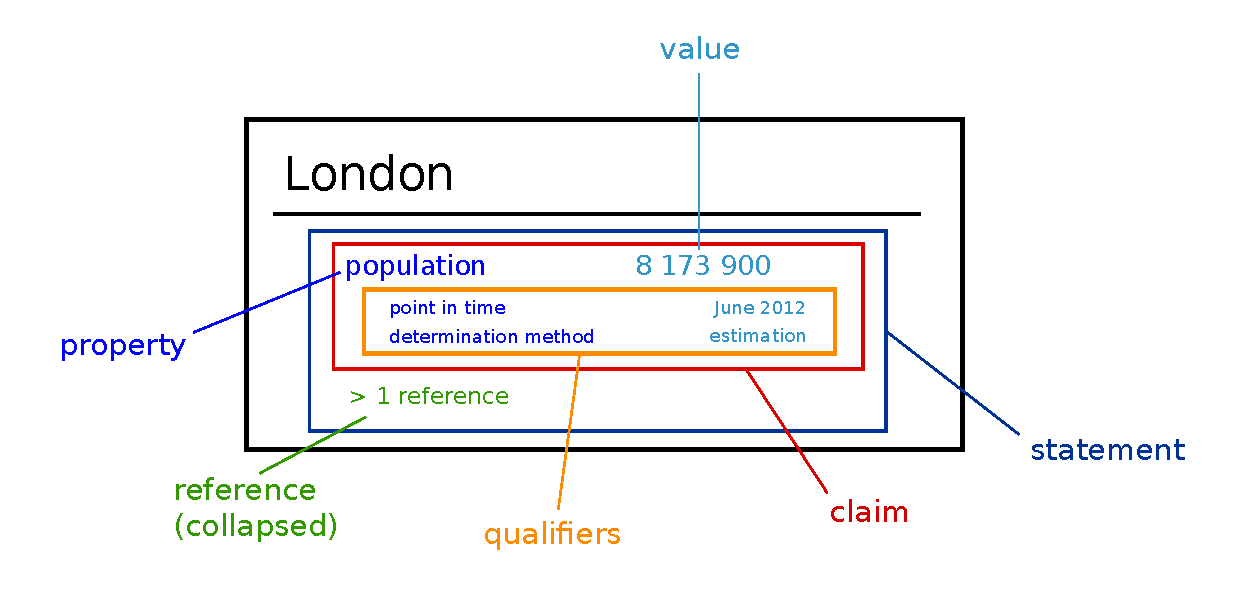
\includegraphics[width=\textwidth]{Wikidata_statement.pdf}

 \vspace*{-0.4cm}
  \begin{itemize}
    \item Wert: (Strict typing) Objekte (Q*), Zeit, URLs, Zahlen, \dots \pause
    \item Qualifikator - z.B. zeitliche Gültigkeit (von - bis) \pause
    \item Referenz kann für jede Aussage angegeben werden. \pause
  \end{itemize}
Es kann mehrere Aussagen gleichen Typs, Referenzen oder Qualifikatoren geben
\end{frame}

\section{Einsatzgebiet von Wikidata für OpenStreetMap}

\subsection{Permanent-IDs}

\begin{frame}{Lösung des Permanent-ID-Problems}

 \vspace*{-0.8cm}
  Problem: Ein Objekt ändert im Laufe seines "`Verbesserungs-Zyklus"' seine ID/URI:

 \vspace*{0.2cm}

  \begin{columns}[c]

    \begin{column}[T]{60mm}
      osm.org/node/790308243 \\
      
\includegraphics[height=15mm]{buschenschank-node.png}
    \end{column} 
    \pause

    \begin{column}[T]{5mm}
       \vspace*{1cm}
      $\Rightarrow$
    \end{column}

    \begin{column}[T]{20mm}
      way/428728632 \\
      
\includegraphics[height=15mm]{buschenschank-way1.png}
    \end{column}
    \pause

    \begin{column}[T]{5mm}
       \vspace*{1cm}
      $\Rightarrow$
    \end{column}

    \begin{column}[T]{20mm}
      relation/6376737 \\
      
\includegraphics[height=15mm]{buschenschank-rel1.png}
    \end{column}

  \end{columns}
 \vspace*{0.2cm}

  \pause

  Wir können uns nicht darauf verlassen, dass der Node als Eckpunkt wiederverwendet wird ... \pause
 \vspace*{0.2cm}
  
  $\Rightarrow$ Ein Tag mit einer 'Permanenten' ID wäre nicht schlecht! \pause
 \vspace*{0.2cm}

  Tag: wikidata = Q42 ?

  $\Rightarrow$ \href{http://overpass-turbo.eu/?w=\%22wikidata\%22\%3D\%22Q1679599\%22+global\&R}{http://overpass-turbo.eu/?w="wikidata"="Q1679599"}

\end{frame}

\subsection{Übersetzung}

{
  \usebackgroundtemplate{ \hfill 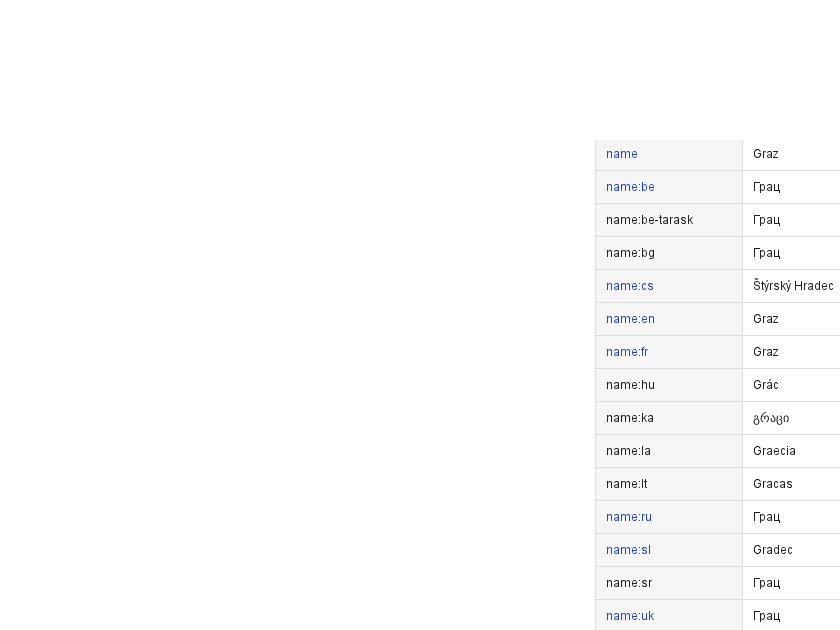
\includegraphics[height=9.5cm]{graz-name-bg.png}}
\begin{frame}{Übersetzungen von OSM-Objekten}
      Jeder kennt das: \\ 
      ~~~ Dutzende name:* - Tags auf Objekten \pause
      \begin{itemize}
        \item Muss man immer extra setzen
        \item Alle Sprachen haben nicht Platz (Tag-Limit)
        \item Gibt's da nicht schon eine Datenbank \\ für Übersetzungen?
        \item Bevor wir die Arbeit doppelt machen, \\ besser bestehendes nutzen! \pause
        \item Idee: Wikipedia-Artikelnamen? \pause
 \vspace*{0.2cm}
        \item Besser: wikidata=* setzen und nutzen! 
      \end{itemize}

\end{frame}
}

\begin{frame}{Übersetzungen von Tags}
  Übersetzungen von OSM-Tags in "`Menschliche"' (Landes-) Sprache ... jeder braucht das!
  \begin{itemize}
    \item Apps und Anwendungsprogramme \pause
    \item Webseiten, die OSM-Attribute darstellen 
      \begin{itemize}
        \item OSM.org: translatewiki.net
      \end{itemize}
      \pause
    \item OSM-Editoren
      \begin{itemize}
        \item iD: Transifex
        \item JOSM: launchpad.net
        \item Potlatch: translatewiki; kein Support für Tag-Übersetzungen!
      \end{itemize}
  \end{itemize}

  Probleme...
  \pause
  \begin{itemize}
    \item Doppelte Arbeit
    \item Inkonsistente Übersetzung
    \item Unsynchron bei neuen Tags
  \end{itemize}

\end{frame}

\section{Praxis}

\subsection{Verlinken von OSM nach Wikidata}

\begin{frame}{Wikidata-Tags}
  Siehe \href{https://wiki.openstreetmap.org/wiki/Proposed\_features/Wikidata}{wiki/Proposed\_features/Wikidata}:
  \begin{itemize}
    \item wikidata = * | \emph{Objekt auf Wikidata} \pause
    \item operator:wikidata = * | \emph{Betreiber, z.B. Q151954 (Lidl) }
    \item brand:wikidata = * 
    \item architect:wikidata = * | \emph{Gebäude-Architekt}
    \item artist:wikidata = * | \emph{Bildhauer}
    \item subject:wikidata = * | \emph{Für z.B. Statuen: Abgebildeter}
    \item name:etymology:wikidata = * | \emph{Wortherkunft, z.B. Böll-Weg}
  \end{itemize}

  \pause
  Frage für die Zukunft: \\
  Bei welchen Tags macht es überhaupt noch Sinn, in der OpenStreetMap Informationen als "`Freitext"' einzutragen und wo ist es Maschinenlesbar auf Wikidata sinnvoller?

\end{frame}

\begin{frame}{OSM-Editoren}

  JOSM: \hfill 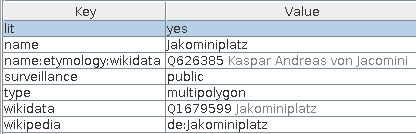
\includegraphics[height=2cm]{jakominiplatz.png}

  \begin{itemize}
    \item Wikipedia-Plugin zeigt Objekt hinter Wikidata-Tags an 
    \item Tags setzen muss man leider noch händisch \dots
  \end{itemize}

  \pause
  iD:
  \begin{itemize}
    \item Wikidata-Tags werden bei setzen eines Wikipedia-Artikels automatisch ergänzt.
  \end{itemize}

\end{frame}


\subsection{Verlinken von Wikidata nach OSM}

\begin{frame}{OSM-Properties in Wikidata}
  Linken auf OSM-Objekte ... tja wie ohne Permanent ID?

 \vspace*{0.2cm}
 Zumindest Relationen sind als "`kompliziertestes"' OSM-Element hinreichend stabil: 
\includegraphics[height=3.5mm]{relation.png}

\begin{itemize}
  \item P402: OpenStreetMap-Relations-ID
  \begin{itemize}
    \item Seine P1630 (URL-Formatierer) zeigt auf https://www.openstreetmap.org/relation/\$1
    \item Wird hauptsächlich für administrative Einheiten (Länder, Gemeinden, \dots) genutzt.
  \end{itemize}

  \pause
  \item Rel-ID händisch eintragen, danach kann man draufklicken.

\end{itemize}



Wie auf andere OSM-Objekte verlinken? Manche werden wohl ewig ein Node bleiben, Bäume z.B. \dots

Wir sollten auf eine Permanent-ID verlinken \dots 


\end{frame}

\begin{frame}{OSM-Tags in Wikidata eintragen \emph{(Übersetzungen!)}}

Wikidata-Einträge/Wikipedia-Artikel mit OSM-Tag verknüpfen:

\begin{itemize}
  \item P1282: OpenStreetMap-Tag oder -Key
  \begin{itemize}
    \item seine P1630 (URL-Formatierer) zeigt auf https://wiki.openstreetmap.org/wiki/\$1
  \end{itemize}
  \item z.B. "`Tag:leisure=hackerspace"' händisch eintragen, danach kann man draufklicken.
\end{itemize}

\pause

Noch ungelöst: Wie bei mehreren Tags für ein Objekt?
 \vspace*{0.2cm}

Man kann zwar mehrere Eigenschaften P1282 eintragen, aber was soll es bedeuten?
\begin{itemize}
  \item Beide Tags müssen am Objekt sein (AND-Verknüpfung)?
  \item Beide Tags sind für dasselbe Objekt gültig (OR-Verknüpfung)?
\end{itemize}

\end{frame}

%\begin{frame}{Hilfe}
%Fragen? 
%\begin{itemize}
%  \item Dokumentation: \href{http://wiki.openstreetmap.org}{wiki.openstreetmap.org}
%  \begin{itemize} 
%    \item Mitmachen? \href{https://wikidata.org}{wikidata.org}
%  \end{itemize}
%\end{itemize}

% \vspace*{-2.8cm}

%\begin{itemize}
%  \item Konferenz: \href{http://stateofthemap.org/}{State of the Map}, 23.-25. September, Brüssel
%\end{itemize}
%\end{frame}

\section{Ende}

\begin{frame}{Vielen Dank für die Aufmerksamkeit!}

  Folien zur FOSSGIS 2016, 4.7.2016, Salzburg
\vspace{1cm}

Erstellt mittels \LaTeX Beamer, Quelltext: \href{https://github.com/species/vortrag-osm-wikidata-fossgis16}{Github/species/vortrag-osm-wikidata-fossgis16}.
\vspace{1cm}

\href{mailto:michael.maier@mailbox.org}{Michael Maier}, OSM-User: species

Twitter: \href{https://twitter.com/osmgraz}{@osmgraz}
\vspace{1cm}

Folien-Quelltext unter: 
\includegraphics[width=1cm]{cc-zero.pdf}. 

\end{frame}


\begin{frame}{Bildnachweise:}

  \begin{columns}[c]
    \begin{column}[T]{20mm}
      
\includegraphics[height=0.5cm]{Hourglass_2.pdf}
    \end{column}
    \begin{column}[T]{90mm}
      CC-BY-SA 3.0, RRZEicons, von \href{https://commons.wikimedia.org/wiki/File:Hourglass_2.svg}{Wikimedia Commons}
    \end{column}
  \end{columns}

\vspace{5mm}
  \begin{columns}[c]
    \begin{column}[T]{20mm}
      
\includegraphics[height=0.5cm]{Road-under-construction.png}
    \end{column}
    \begin{column}[T]{90mm}
      CC-0, von \href{https://commons.wikimedia.org/wiki/File:Road-under-construction.png}{Wikimedia Commons}
    \end{column}
  \end{columns}

\vspace{5mm}
  \begin{columns}[c]
    \begin{column}[T]{20mm}
      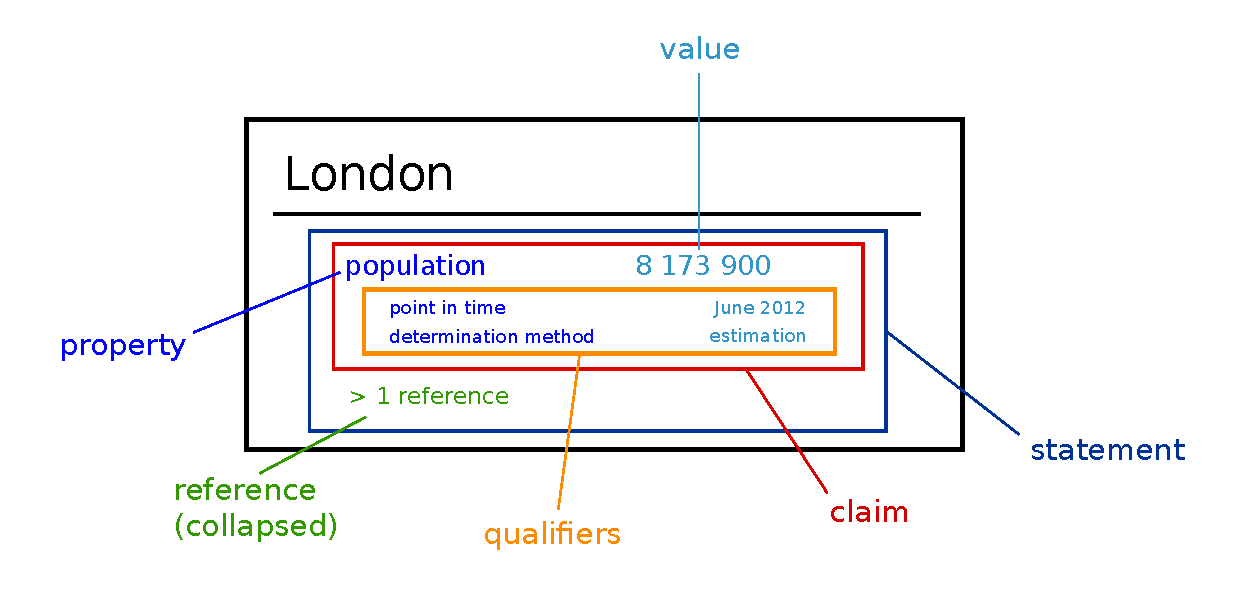
\includegraphics[width=20mm]{Wikidata_statement.pdf}
    \end{column}
    \begin{column}[T]{90mm}
      Wikidata-Statement: CC-BY-SA 3.0, von \href{https://commons.wikimedia.org/wiki/File:Wikidata_statement.svg}{Wikimedia Commons}
    \end{column}
  \end{columns}

\vspace{5mm}
  \begin{columns}[c]
    \begin{column}[T]{20mm}
      Wikimedia \& Wikidata Logo
    \end{column}
    \begin{column}[T]{90mm}
      CC-0 Wikimedia Foundation
    \end{column}
  \end{columns}

\end{frame}

\end{document}
